En este capítulo se describe toda la información que manejará el sistema. Se describen todos los datos que serán entradas y salidas mediante la descripción de Entidades, atributos y sus relaciones. Cada entidad se representa como una clase y cada fila de la entidad le corresponde un atributo en su clase.Las relaciones entre clases se modelan utilizando conceptos como

Participación, Composición, Agregación y Generalización. Para poder llevar a cabo la relación de atributos y clases con el negocio, se utiliza la notación UML2.0 especificada por la \href{www.omg.org}{OMG}.

%--------Modelo Estructural del Proceso de Infraestructura------------------%
\section{Modelo Estructural de Gestión de Infraestructura}
	%En la figura \ref{fig:infraestructuraDC} se muestra la estructura de información que manejará el \refElem{Calmecac} para llevar a cabo la gestión de unidades académicas, edificios y espacios.

\begin{figure}[hbtp!]
	\begin{center}
%				\fbox{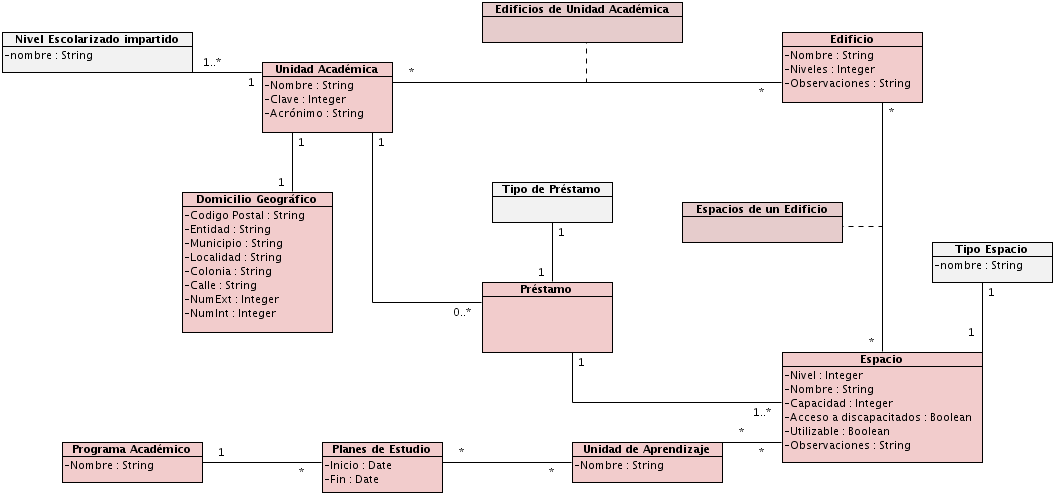
\includegraphics[width=\textwidth]{negocio/images/Modelodeinformacion_Procesodeinfraestructura_version_dos}}
%		\caption{Diagrama de Clases de Infraestructura}
%		\label{fig:infraestructuraDC}
	\end{center}
\end{figure}

%----------------------Entidades-------------------------------------------%

%=====Unidad Académica=====%
%\begin{cdtEntidad}{unidadAcademica}{Unidad Académica}
%	\brAttr{nombre}{Nombre}{Frase}{Es el nombre asignado a una unidad académica de acuerdo a los programas académicos que se imparten en ella}{\datRequerido}
%	\brAttr{clave}{Clave}{Entero}{Es la clave con la que una unidad académica puede ser identificada de otras}{\datRequerido}
%	\brAttr{acronimo}{Acrónimo}{Palabra}{Son las siglas con las que se pueden identificar las diferentes unidades académicas}{\datRequerido}
%	%----------------------------------
%	\cdtEntityRelSection
%	\brRel{\brRelAgregation}{\refElem{nivelEscolarizadoImpartido}}{Una \refElem{unidadAcademica} tiene  al menos un \refElem{nivelEscolarizadoImpartido}}
%	\brRel{\brRelComposition}{\refElem{domicilioGeografico}}{Una \refElem{unidadAcademica} reside en un \refElem{domicilioGeografico}}
%	\brRel{\brRelComposition}{\refElem{edificio}}{Una \refElem{unidadAcademica} tiene \refElem{edificio}}
%\end{cdtEntidad}



\input{negocio/informacionHorarios}
%En la figura \ref{fig:infoProfesores} se puede observar la información que el \refElem{Calmecac} utilizará de acuerdo a los servicios web proporcionados por el \refElem{SIEE}.%Verificar
%
%\begin{figure}[hbtp!]
%	\begin{center}
%	\fbox{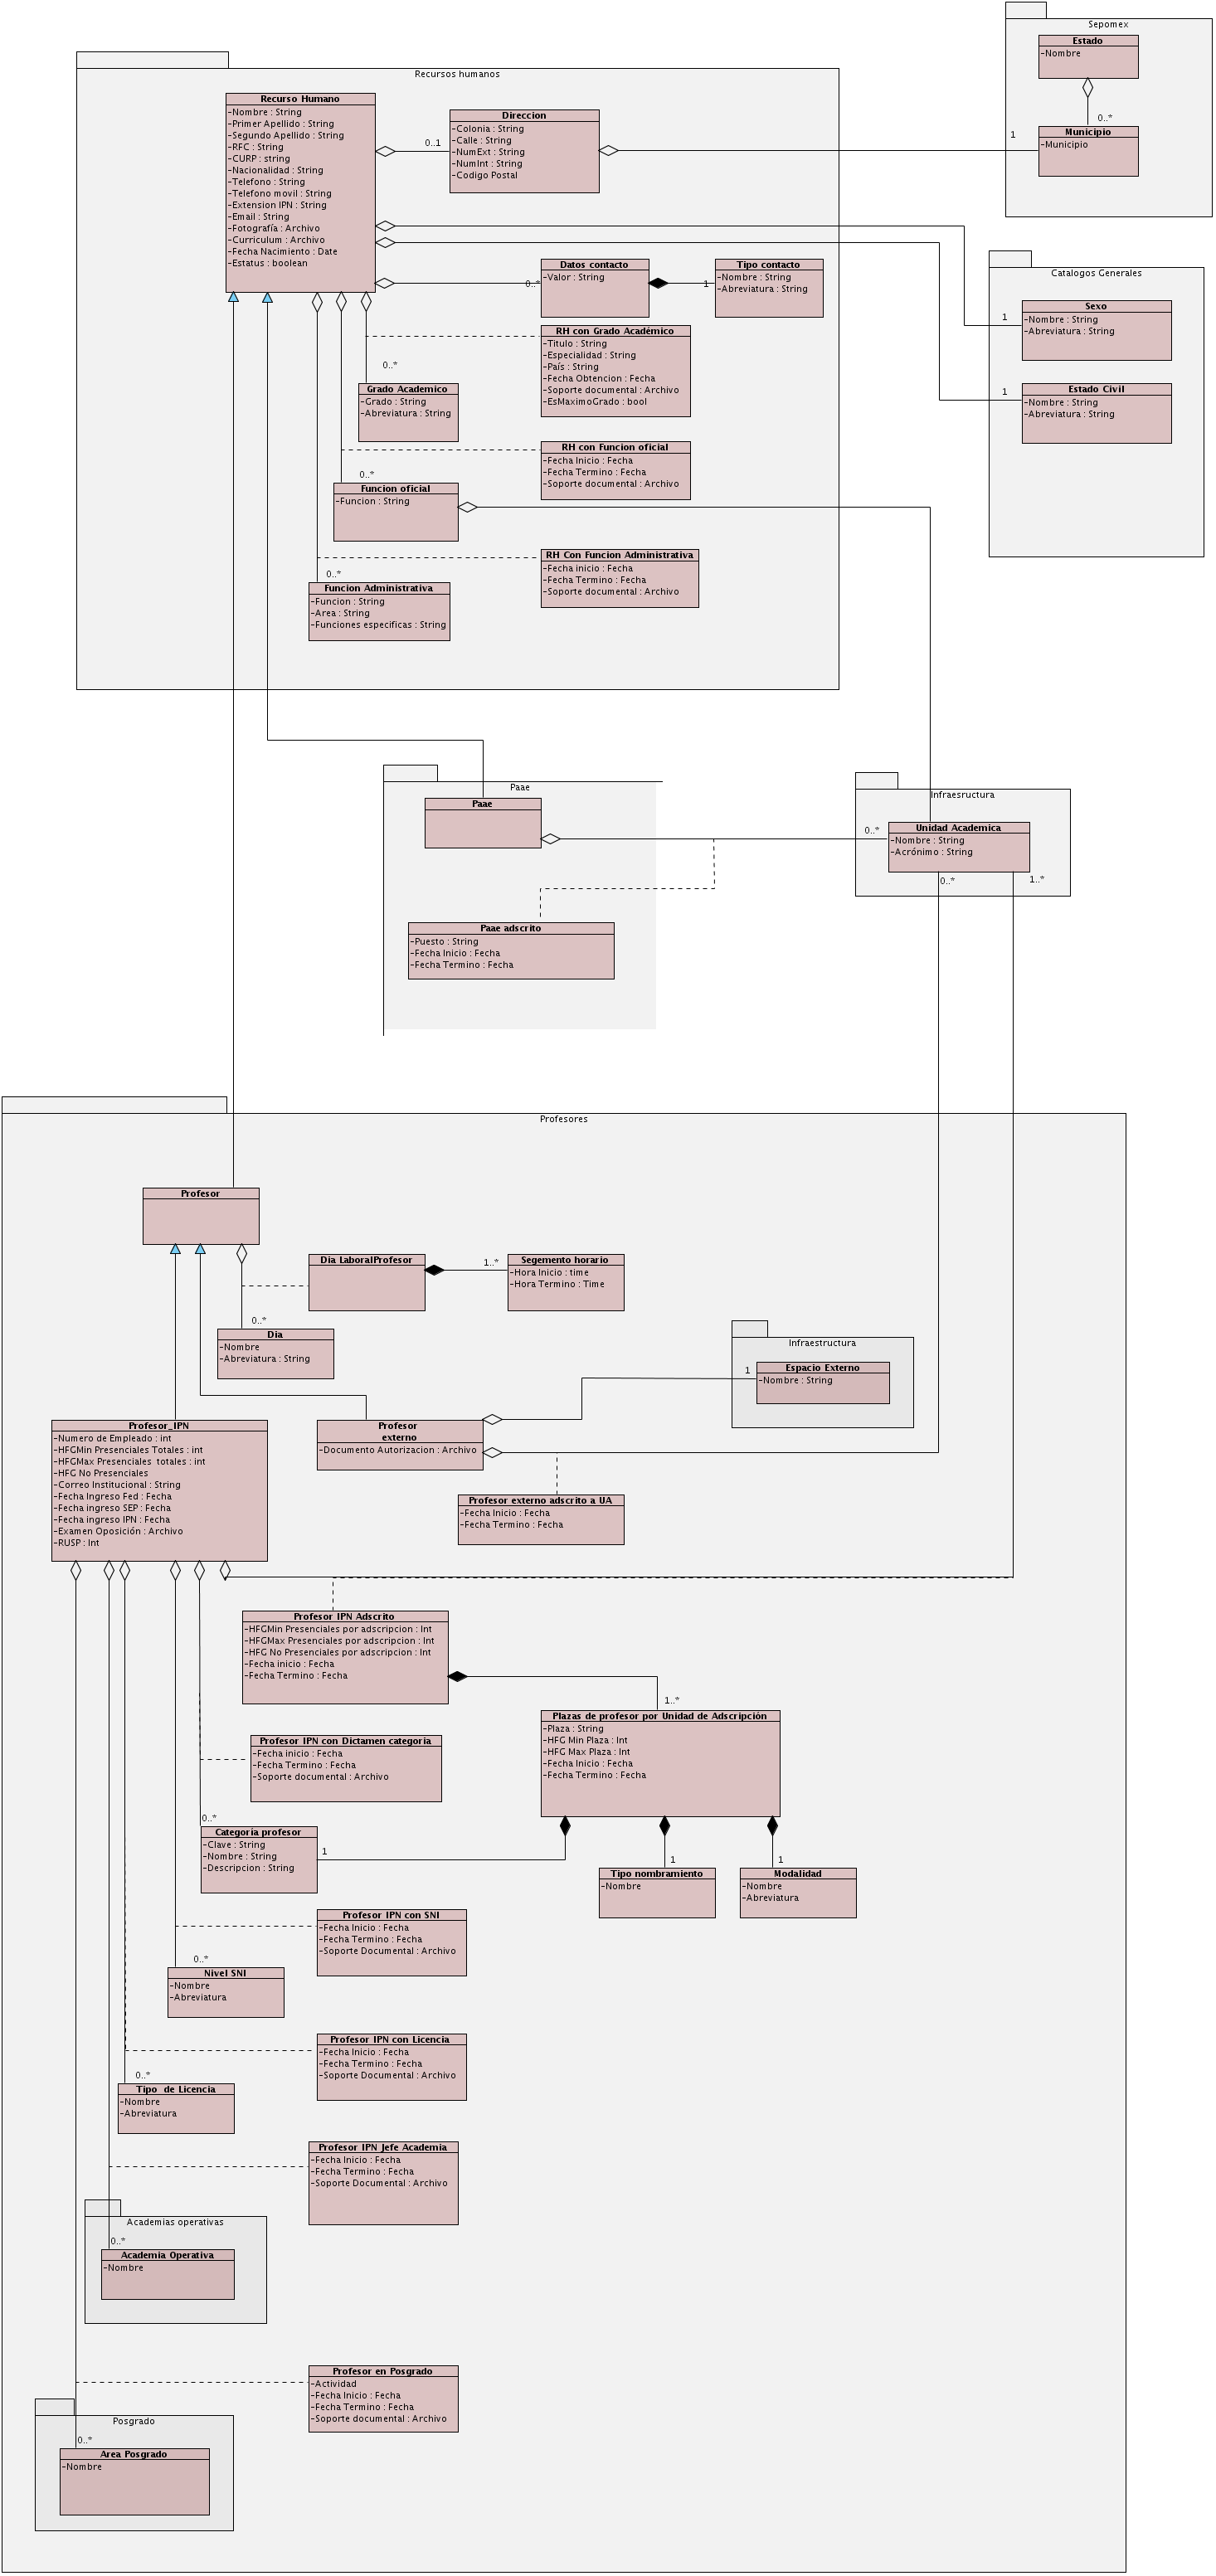
\includegraphics[width=\textwidth]{negocio/images/ModeloDeInformacion_Profesores}}
%		\label{fig:infoProfesores}
%		\caption{Modelo de Información de Profesores}
%	\end{center}
%\end{figure}

%===================================Paquete RECURSOS Humanos
%----------------------------------Recurso Humano--------------------------------------
\begin{cdtEntidad}[Es una persona que forma parte del Instituto Politécnico Nacional y que se encarga de realizar actividades administrativas y de gestión en las Unidades Académicas, Unidades Administrativas, Centros de Investigación o en los Órganos Consultivos. Su relación con el Instituto puede estar determinada por un contrato o por un convenio con una Unidad de Adscripción en específico.]{RecursoHumano}{Recurso Humano}
	\brAttr{nombre}{Nombre}{frase}{Representa la palabra o conjunto de palabras con las que se designan y se distinguen a una persona que labora en el Instituto.}{\datRequerido}
	\brAttr{primerApellido}{Primer apellido}{frase}{Representa la palabra o conjunto de palabras que sigue al nombre de pila de una persona y que se transmite de padres a hijos.}{\datRequerido}
	\brAttr{segundoApellido}{Segundo apellido}{frase}{Representa la palabra o conjunto de palabras que sigue al primer apellido de una persona y que se transmite de padres a hijos.}{\datOpcional}
	\brAttr{RFC}{RFC}{palabra}{Representa la clave alfanumérica compuesta de 13 caracteres que permite cumplir con las obligaciones que la ley establece para el pago de impuestos. En el Instituto es un mecanismo que ayuda a identificar a una persona que labora o apoya en las actividades académicas y administrativas. }{\datRequerido}
	\brAttr{CURP}{CURP}{palabra}{Representa la clave alfanumérica compuesta de 18 caracteres que permite identificar a un ciudadano residente de México. En el Instituto es otro de los mecanismos que ayudan a identificar a una persona que labora o apoya en las actividades académicas y administrativas.}{\datRequerido}
	\brAttr{fechaDeNacimiento}{Fecha de Nacimiento}{fecha}{Es la fecha que, en el Acta de Nacimiento de una persona, establece el día en que nació.}{\datRequerido}
	\brAttr{fechaDeUltimaActualizacion}{Fecha de última actualización}{fecha}{Indica la fecha en la que en el sistema se llevo a cabo una modificación o actualización en los datos o relaciones de una persona con otras entidades.}{\datOpcional}
	\brAttr{numeroDeEmpleado}{Número de Empleado}{entero}{Secuencia de dígitos numéricos que se utiliza para identificar a un profesor contratado por la Dirección Capital Humano. Su expresión regular es : $ [0-9]\{6,\}$. Este número no le es otorgado al personas que es contratado por honorarios o como visitante.}{\datOpcional}
	\brAttr{Activo}{Activo}{booleano}{Dato que representa si un recurso humano del Instituto se encuentra: \begin{Citemize}
			\item Activo -- Indica que el Recurso Humano se encuentra realizando actividades académicas y/o administrativas en el momento de su consulta.
			\item Inactivo -- Indica que el Recuro Humano no se encuentra realizando actividades académicas y/o administrativas en el momento de su consulta.
	\end{Citemize}}{\datOpcional}
	\brAttr{sexo}{Sexo}{Sexo}{Indica la sexualidad de un recurso humano con base en su acta de nacimiento.}{\datOpcional}
	\brAttr{pais}{País}{Pais}{Indica la nacionalidad de un recurso humano y que indica su relación con un país por medio de un gentilicio.}{\datOpcional}
	\cdtEntityRelSection
	\brRel{\brRelAgregation}{\refElem{tdGradoAcademico}}{Un Recurso Humano ha adquirido una o varias distinciones académicas a lo largo de su vida que ayudan a determinar, en algunos casos su categoría o posición dentro del Instituto así como su asignación de exposiciones para impartir los contenidos de una o varias Unidades de Aprendizaje.}
	\brRel{\brRelComposition}{\refElem{Documento}}{Un Recurso Humano adquiere una o más pruebas materiales que acreditan un grado, logro académico o algún otro documento en donde se establezca un aspecto relevante para la asignación de labores.}
	\brRel{\brRelComposition}{\refElem{ContactoDeRecursoHumano}}{Un Recurso Humano tiene uno o varios medios de contacto que se pueden utilizar para comunicarse con el o para enviarle notificaciones.}
	\brRel{\brRelAgregation}{\refElem{UnidadDeAdscripcion}}{Un Recurso Humano puede estar asignado a más de una Unidad de Adscripción en donde desempeña las labores designadas por un contrato o por un convenio.}
	\brRel{\brRelGeneralization}{\refElem{ProfesorIPN}}{Un Profesor que labore en el Instituto es un Recurso Humano que es considerado para la designación de labores docentes y de investigación en una o más unidades de adscripción.}
\end{cdtEntidad}

\begin{cdtEntidad}[Es uno de los métodos con los que se cuenta para comunicarse o ubicar a una persona y mantenerle informado acerca de noticias, notificaciones y cambios en los distintos procesos del Instituto que así lo requieran.]{ContactoDeRecursoHumano}{Contacto de Recurso Humano}
	%=======Atributos
	\brAttr{contacto}{Contacto}{palabra}{Es el conjunto de caracteres que representan a un mecanismo que se utiliza para poder comunicarse con un recurso humano.}{\datRequerido}
	\brAttr{contactoAuxiliarA}{Contacto Auxiliar A}{palabra}{Es un carácter o conjunto de caractere que tienen la utilidad de almacenar información adicional.}{\datOpcional}
	\brAttr{contactoAuxiliarB}{Contacto Auxiliar B}{palabra}{Es un carácter o conjunto de caractere que tienen la utilidad de almacenar información adicional.}{\datOpcional}
	\brAttr{tipoDeContacto}{Tipo de Contacto}{TipoDeContacto}{Se utiliza para especificar y clasificar al contacto por sus características.}{\datRequerido}
	%======Relaciones
	\cdtEntityRelSection
	\brRel{\brRelComposition}{\refElem{RecursoHumano}}{Un recurso humano tiene uno o varios medios de contacto que se pueden utilizar para comunicarse con el o para enviarle notificaciones.}
\end{cdtEntidad}

%---------------------------------------RHGrado Académico--------------------------------------------%
\begin{cdtEntidad}[En es el resultado de la relación entre \refElem{RecursoHumano} y \refElem{tdGradoAcademico} y tiene como propósito almacenar todas aquellas distinciones académicas que un Recurso Humano ha adquirido con el paso de tiempo y que se utiliza como apoyo al definir la asignación de exposiciones de Unidades de Aprendizaje a Grupos.]{RecursoHumanoConGradoAcademico}{Recurso Humano con Grado Académico}
	%====Atributos
	\brAttr{titulo}{Titulo}{frase}{Conjunto de palabras que representan un grado y el programa de estudios  adquirido por un recurso humano.}{\datRequerido}
	\brAttr{fechaDeObtencion}{Fecha de Obtención}{fecha}{Indica el día en que un grado académico se adquiere. Está fecha puede encontrarse en el documento que avala la adquisición de un grado del Recurso Humano.}{\datRequerido}	
	\brAttr{fechaDeExpedicion}{Fecha de Expedición}{fecha}{Indica el día en que el documento que avala la adquisición de un grado es emitido.}{\datOpcional}	
	\brAttr{esUltimoGrado}{Es Último Grado}{booleano}{Indica si el grado adquirido es el máximo obtenido por el \refElem{RecursoHumano} tomando como referencia otras distinciones adquiridas, si las tiene, o en la escala del nivel educativo correspondiente.}{\datRequerido}	
	\brAttr{pais}{País}{Pais}{Indica el país de procedencia del grado obtenido por el recurso humano.}{\datRequerido}	
	\brAttr[Entidad]{documento}{Documento}{Documento}{Un grado académico adquirido por un recurso humano es avalado por una prueba material en el que se especifica la conclusión de un programa de estudios. }{\datRequerido}
\end{cdtEntidad}

\begin{cdtEntidad}[Es la prueba material que contiene información acerca de un hecho académico o laboral de un Recurso Humano y que es emitida por instituciones o personas físicas o morales.]{Documento}{Documento}
	\brAttr{nombre}{Nombre}{frase}{Es la palabra o el conjunto de palabras que tienen como propósito identificar una prueba material que contiene información acerca de un hecho académico o laboral de un Recurso Humano.}{\datRequerido}		
	\brAttr{fechaDeInicio}{Fecha de Inicio}{fecha}{Indica el día en que inicia la validez de una prueba material que sirve para especificar un nombramiento, un logro académico o una actividad.}{\datRequerido}
	\brAttr{fechaDeFin}{Fecha de Fin}{fecha}{Indica el día en que concluye la validez de una prueba material que sirve para especificar un nombramiento, un logro académico o una actividad.}{\datOpcional}
	\brAttr{documento}{Documento}{archivo}{Es un conjunto de datos que guardan el contenido de una prueba material que avala un suceso o un hecho acontecido en la trayectoria académica o de docencia de un Recurso Humano. }{\datOpcional}
	\cdtEntityRelSection
	\brRel{\brRelComposition}{\refElem{RecursoHumano}}{Un Recurso Humano adquiere una o más pruebas materiales que acreditan un grado, logro académico o algún otro documento en donde se establezca un aspecto relevante para la asignación de labores.}
	\brRel{\brRelComposition}{\refElem{ProfesorIPN}}{Un Profesor del Instituto adquiere un documento que avala la presentación y aprobación del examen correspondiente al concurso de oposición. }
	\brRel{\brRelComposition}{\refElem{RecursoHumanoConGradoAcademico}}{Un grado académico adquirido por un recurso humano es avalado por una prueba material en el que se especifica la conclusión de un programa de estudios.}
	\brRel{\brRelComposition}{\refElem{DictamenDeCategoria}}{Un Profesor del Instituto tiene una prueba material que le soporta una categoría la cual indica la carga frente a grupo que debe cubrir.}
\end{cdtEntidad}

\begin{cdtEntidad}[Es una un elemento que pertenece a la estructura organizacional del Instituto, mismo que le define las funciones orgánicas y la destinación de recursos que apoyen al cumplimiento de sus objetivos.]{UnidadDeAdscripcion}{Unidad de Adscripción}
	\brAttr{nombre}{Nombre}{frase}{Es la palabra o conjunto de palabras que identifican a una Unidad de Adscripción.}{\datRequerido}
	\brAttr{clave}{Clave}{palabra}{Es la secuencia de caracteres que identifican a una Unidad de Adscripción.}{\datOpcional}
	\brAttr{zonaPagadora}{Zona Pagadora}{palabra}{Es una clave numérica, la cual se valida con la expresión regular $[0-9]\{4\}$. Representa el lugar destinado para la entrega de pagos a los empleados del Instituto.}{\datOpcional}
	\brAttr{tipoDeUnidadAdscripcion}{Tipo de Unidad de Adscripción}{TipoDeUnidadAdscripcion}{Se utiliza para especificar y clasificar a la Unidad de Adscripción de acuerdo a sus funciones y objetivos. }{\datRequerido}	
	\cdtEntityRelSection
	\brRel{\brRelComposition}{\refElem{UnidadDeAdscripcion}}{Una Unidad de Adscripción puede estar compuesta de otras Unidades de Adscripción. Por ejemplo:
	\begin{Citemize}
		\item Las unidades de adscripción División de Gestión y Calidad Educativa y la División de Innovación Académica están dentro de la unidad de adscripción Dirección de Educación Superior.
		\item Las unidades de adscripción División de Admisión y Control Escolar y la División de Registro y Certificación de Estudios están dentro de la unidad de adscripción Dirección de Administración Escolar.
	\end{Citemize}}
	\brRel{\brRelAgregation}{\refElem{RecursoHumano}}{Un Recurso Humano del Instituto puede pertenecer a más de una Unidad de Adscripción.}
\end{cdtEntidad}

\begin{cdtEntidad}[Es el vínculo establecido entre un recurso humano y una o más unidades de adscripción en el cual se especifican las funciones laborales del recurso para un periodo de tiempo determinado por un contrato o un convenio. ]{Adscripcion}{Adscripción}
	\brAttr{fechaDeInicio}{Fecha de Inicio}{fecha}{Es el día en el que se especifica el inicio de las labores de un recurso humano en una unidad de adscripción.}{\datRequerido}
	\brAttr{fechaDeFin}{Fecha de Fin}{fecha}{Es el día en el que se especifica la conclusión de labores de un recurso humano en una unidad de adscripción.}{\datOpcional}
	\brAttr{tipoDeRecurso}{Tipo de Recurso}{TipoDeRecurso}{Se utiliza para especificar y clasificar a la adscripción del recurso humano de acuerdo a su forma de contratación y de sus funciones en la Unidad de Adscripción.}{\datRequerido}
	\brAttr{nivelAcademico}{Nivel Académico}{NivelAcademico}{Indica a cuál nivel corresponde la adscripción de un recurso humano.}{\datRequerido}
	\cdtEntityRelSection
	\brRel{\brRelAgregation}{\refElem{tdRolFuncional}}{La adscripción de un recurso humano tiene asociado uno o más roles que definen las funciones y permisos a los que se tendrá acceso.}
	\brRel{\brRelGeneralization}{\refElem{AdscripcionIPN}}{La adscripción de un recurso humano que realiza labores de docencia en el Instituto determina el número de exposiciones que debe realizar frente a grupo.}
\end{cdtEntidad}

\begin{cdtEntidad}[Es el vínculo establecido entre un \refElem{RecursoHumano} contratado por la Dirección de Capital Humano y que realiza labores de docente  en una \refElem{UnidadDeAdscripcion} en la cual se determina el número de horas máximas, mínimas, de nombramiento y no presenciales que se deben cubrir por plaza.]{AdscripcionIPN}{Adscripción IPN}
	\brAttr{HFGMinimas}{Horas Frente a Grupo Mínimas}{entero}{Es el conjunto de dígitos que representan el mínimo de horas que el recurso humano debe ser asignado en una unidad de adscripción para realizar las exposición de los contenidos de una o más Unidades de Aprendizaje ofertadas para un periodo. Estas horas están determinadas por el número de plazas adquiridas por el recurso humano adscrito.}{\datRequerido}
	\brAttr{HFGMaximas}{Horas Frente a Grupo Máximas}{entero}{Es el conjunto de dígitos que representan el máximo de horas que el recurso humano debe ser asignado en una unidad de adscripción para realizar las exposición de los contenidos de una o más Unidades de Aprendizaje ofertadas para un periodo. Estas horas están determinadas por el número de plazas adquiridas por el recurso humano adscrito.}{\datRequerido}
	\brAttr{HFGNoPresenciales}{Horas Frente a Grupo No Presenciales}{entero}{Es el conjunto de dígitos que representan las horas que el recurso humano debe ser asignado para la modalidad no escolarizada. Estas horas están determinadas por el número de plazas adquiridas por el recurso humano adscrito.}{\datRequerido}
	\brAttr{HorasDeNombramiento}{Horas de Nombramiento}{entero}{Es el dígito que representa las horas que el recurso humano debe ser asignado de acuerdo a su nombramiento. Estas horas están determinadas por el número de plazas adquiridas por el recurso humano adscrito.}{\datRequerido}
	\cdtEntityRelSection
	\brRel{\brRelComposition}{\refElem{Plaza}}{El Recurso Humano que esta contratado para realizar labores de docencia en una Unidad de Adscripción cubre un número de plazas.}
	\brRel{\brRelGeneralization}{\refElem{Adscripcion}}{Una Adscripción al Politécnico es una Adscripción determinada por el vinculo entre un Recurso Humano que realiza exposiciones de una Unidad de Aprendizaje en un Grupo.}
\end{cdtEntidad}


\begin{cdtEntidad}[Es un elemento en el que se definen aspectos laborales de la Adscripción de un Recurso Humano con una Unidad de Adscripción tales como el rango de fechas que indican la validez de la plaza, el número de horas mínimas y máximas frente a grupo que deben ser asignadas para realizar exposiciones de contenido de las Unidades de Aprendizaje, la categoría asignada y las horas de nombramiento.]{Plaza}{Plaza}
	\brAttr{HFGMinimas}{Horas Frente a Grupo Mínimas}{entero}{Es el conjunto de dígitos que representan el mínimo de horas por plaza que el recurso humano debe ser asignado en una unidad de adscripción para realizar las exposición de los contenidos de una o más unidades de aprendizaje ofertadas para un periodo. }{\datRequerido}	
	\brAttr{HFGDeNombramiento}{Horas Frente a Grupo de Nombramiento}{entero}{Es el conjunto de dígitos que representan las horas por plaza que el recurso humano debe ser asignado de acuerdo a su nombramiento.}{\datOpcional}
	\brAttr{fechaDeInicio}{Fecha de Inicio}{fecha}{Indica el día en que la plaza inicia su periodo de validez.}{\datRequerido}
	\brAttr{fechaDeFin}{Fecha de Fin}{fecha}{Indica el día en que la plaza concluye su periodo de validez.}{\datOpcional}
	\brAttr{HFGMaximas}{Horas Frente a Grupo Máximas}{entero}{Es el conjunto de dígitos que representan el máximo de horas por plaza que el recurso humano debe ser asignado en una Unidad de Adscripción para realizar las exposición de los contenidos de una o más Unidades de Aprendizaje ofertadas para un periodo.}{\datRequerido}	
	\brAttr{categoria}{Categoría}{Categoria}{Especifica a qué nivel pertenece la plaza del Recurso Humano indicando el número de horas que debe cubrir frente a un grupo para obtener su carga máxima. }{\datRequerido}
	\brAttr{tipoDeNombramiento}{Tipo de Nombramiento}{TipoDeNombramiento}{Indica el número de horas que un Recurso Humano contratado por la Dirección de Capital Humano del Instituto y asociado a una Unidad de Adscripción como docente debe cubrir de acuerdo a la plaza adquirida.}{\datRequerido}
	\brAttr{modalidad}{Modalidad}{Modalidad}{Indica para qué Modalidad se deberán asignar las horas de la Plaza.}{\datRequerido}
	\cdtEntityRelSection
	\brRel{\brRelComposition}{\refElem{AdscripcionIPN}}{El Recurso Humano que esta contratado para realizar labores de docencia en una Unidad de Adscripción cubre un número de plazas.}
\end{cdtEntidad}

\begin{cdtEntidad}[Es un recurso humano cuya relación con el Instituto se encuentra definida por uno o varios contratos en el que se establecen las horas en las que debe cubrir su carga académica o fungir como apoyo en prácticas y/o en la teoría de las Unidades de Aprendizaje en las que se encuentra asignado dentro de una Estructura Educativa.]{ProfesorIPN}{Profesor del Instituto}
	\brAttr{fechaDeIngresoSEP}{Fecha de Ingreso a la SEP}{fecha}{Indica el día en que el Profesor se incorporó a la Secretaría de Educación Pública.}{\datOpcional}
	\brAttr{fechaDeIngresoIPN}{Fecha de Ingreso al Instituto}{fecha}{Indica el día en que el Profesor se incorporó al Instituto Politécnico Nacional como docente.}{\datOpcional}
	\brAttr{RUSP}{RUSP}{entero}{Indica el número del Registro de Servidores Públicos del Gobierno Federal que le fue asignado.}{\datOpcional}
	\brAttr{turno}{Turno}{Turno}{Indica al segmento de horas de un día en que un profesor del Instituto labora en una unidad de adscripción.}{\datRequerido}	
	\brAttr{tipoDeNombramiento}{Tipo de Nombramiento}{TipoDeNombramiento}{Indica el si el conjunto de horas que se deben asignar al Profesor del Instituto son de su propiedad o si las horas por las cual fue contratado deben cubrir algún tipo de incidencia. }{\datRequerido}	
	\cdtEntityRelSection	
	\brRel{\brRelAgregation}{\refElem{tdDia}}{Un profesor del Instituto labora a la semana un conjunto de días y horas con lo que se define así un horario en el que desempeña labores de docente y/o investigación.}	
	\brRel{\brRelComposition}{\refElem{Documento}}{Un Profesor del Instituto adquiere un documento que avala la presentación y aprobación del examen correspondiente al concurso de oposición. }
	\brRel{\brRelComposition}{\refElem{DictamenDeCategoria}}{Un Profesor del Instituto tiene una o más categorías que determinan el número de horas que debe cubrir frente a grupo para obtener la carga máxima de su plaza.}
	\brRel{\brRelGeneralization}{\refElem{RecursoHumano}}{Un profesor que labore en el Instituto es un recurso humano que es considerado para la designación de labores docentes y de investigación en una o más unidades de adscripción.}
\end{cdtEntidad}

\begin{cdtEntidad}[Es la entidad en la que se encuentran definidas las secciones de varios días de la semana en los que un profesor realiza actividades académicas como impartir clase o realizar actividades complementarias así como de investigación.\\]{Horario}{Horario}
	\brAttr{horaDeInicio}{Hora de Inicio}{hora}{Indica la hora en un día en que el Profesor inicia un un segmento de actividades académicas de un día laboral.}{\datRequerido}
	\brAttr{horaFinal}{Hora Final}{hora}{Indica la hora en que el Profesor concluye un segmento de actividades académicas de un día laboral}{\datRequerido}
\end{cdtEntidad}

\begin{cdtEntidad}[Es el resultado de la relación entre Adscripción y Rol Funcional. Esta relación especifica las diferentes funcionalidades a las que un Recurso Humano tiene acceso en el Sistema durante un rango especificado de fechas.]{Funcion}{Función}
	\brAttr{fechaDeInicio}{Fecha de Inicio}{fecha}{Indica el día en que una funcionalidad del Sistema puede comenzar a ser usada por un Recurso Humano adscrito.}{\datRequerido}	
	\brAttr{fechaDeFin}{Fecha de Fin}{fecha}{Indica el día en que una funcionalidad del Sistema dejará de ser válida para su uso por un Recurso Humano adscrito.}{\datRequerido}
\end{cdtEntidad}

\begin{cdtEntidad}[Es la entidad en la que se especifican todas las categorías que un Profesor del Instituto tiene y que sirven para la asignación de horas máximas que debe cubrir frente a un grupo realizando exposiciones de los contenidos de las Unidades de Aprendizaje Ofertadas en uno o más periodos.]{DictamenDeCategoria}{Dictamen de Categoría}
	\brAttr{fechaDeInicio}{Fecha de Inicio}{fecha}{Indica el día en que una categoría asignada a un Profesor del Instituto inicia su periodo de validez y que sirve para la asignación de horas frente a grupo. }{\datRequerido}
	\brAttr{categoria}{Categoría}{Categoria}{Indica el nivel al que pertenece un dictamen de un Profesor al que se le ha asignado una categoría. }{\datRequerido}
	\cdtEntityRelSection
	\brRel{\brRelComposition}{\refElem{Documento}}{Un Profesor del Instituto tiene una prueba material que le soporta una categoría la cual indica la carga frente a grupo que debe cubrir.}
	\brRel{\brRelComposition}{\refElem{ProfesorIPN}}{Un Profesor del Instituto tiene una o más categorías que determinan el número de horas que debe cubrir frente a grupo para obtener la carga máxima de su plaza.}
\end{cdtEntidad}




%En la figura \ref{fig:infoAlumno} se puede observar un modelado de los datos que serán utilizados en el Calmecac para indicar las relaciones que un Alumno dentro del Instituto tiene y que se van generando a lo largo de su trayectoria escolar, así como de su información personal.


%\begin{figure}
%	\fbox{\includegraphics[width=\textwidth]{../negocio/images/informacion-Alumno}}
%	\label{fig:infoAlumno}
%	\caption{Modelo de Información del Alumno}
%\end{figure}


%===Entidad Alumno
\begin{cdtEntidad}[Es alumno aquella persona que al concluir un proceso de inscripción en el Instituto recibe un número de boleta y un documento que indica su asignación a un programa académico en una unidad académica en cualquier nivel educativo y modalidad educativa.]{Alumno}{Alumno}%
	\brAttr{nombre}{Nombre}{frase}{Representa la palabra o conjunto de palabras con las que se designan y se distinguen a una persona que se encuentra inscrita en algún programa académico que se imparta en cualquier nivel educativo y modalidad educativa que ofrece el Instituto Politécnico Nacional.}{\datRequerido}
	\brAttr{primerApellido}{Primer Apellido}{frase}{Representa la palabra o conjunto de palabras que sigue al nombre de pila de una persona y que se transmite de padres a hijos.}{\datRequerido}
	\brAttr{segundoApellido}{Segundo Apellido}{frase}{Representa la palabra o conjunto de palabras que sigue al primer apellido de una persona y que se transmite de padres a hijos.}{\datOpcional}
	\brAttr{curp}{CURP}{palabra}{Representa la clave alfanumérica compuesta de 18 caracteres que permite identificar a un ciudadano residente de México. En el Instituto es otro de los mecanismos que ayudan a identificar a un Alumno.}{\datRequerido}
	\brAttr{fechaDeNacimiento}{Fecha de Nacimiento}{fecha}{Es la fecha que, en el Acta de Nacimiento de un alumno, establece el día en que nació.}{\datRequerido}
	\brAttr{fechaDeUltimaActualizacion}{Fecha de Última Actualización}{fecha}{Indica la fecha en la que en el sistema se llevo a cabo una modificación o actualización en los datos o relaciones de un alumno con otras entidades.}{\datOpcional}
	\brAttr{fotografia}{Fotografía}{archivo}{Es una imagen que contiene el rostro del alumno.}{\datOpcional}
	\brAttr{lugarDeNacimiento}{Lugar de nacimiento}{Entidad}{Indica de qué parte de la República Mexicana proviene el Alumno si su nacionalidad es mexicana.  En otro caso este atributo quedará vacío para indicar que el Alumno es extranjero}{\datOpcional}
	\brAttr[Entidad]{domicilio}{Domicilio}{Domicilio}{Indica el lugar dentro de un estado de la República Mexicana en la que el alumno reside.}{\datRequerido}
	\brAttr{sexo}{Sexo}{Sexo}{Indica la sexualidad de un alumno con base en su acta de nacimiento.}{\datRequerido}
	\brAttr{pais}{País}{Pais}{Indica la nacionalidad de un alumno y sirve para especificar el atributo \refElem{Alumno.entidad} en caso de que sea Mexicano o dejarlo vacío en cualquier otro caso.}{\datRequerido}
	\brAttr[Entidad]{informacionMedica}{Información Médica}{InformacionMedica}{Un alumno posee un conjunto de datos que especifican su estado de salud, así como su afiliación correspondiente con el Instituto Mexicano del Seguro Social.}{\datRequerido}
	\cdtEntityRelSection
	\brRel{\brRelComposition}{\refElem{DocumentoDeIdentidad}}{Un alumno posee uno o más documentos que comprueban su identidad así como su nacionalidad, su fecha de nacimiento, su mayoría de edad entre otros aspectos.}
	\brRel{\brRelComposition}{\refElem{ContactoDeAlumno}}{Un alumno posee varios mecanismos que utiliza para comunicarse o para ser informado acerca de acontecimientos relacionados a su trayectoria académica en el Instituto.}
	\brRel{\brRelAgregation}{\refElem{tdTipoDeDeporte}}{Un alumno puede o no realizar actividades físicas.}
	\brRel{\brRelComposition}{\refElem{ContactoPersonal}}{Un alumno esta relacionado con un conjunto de personas a las que generalmente se les atribuye un grado de responsabilidad en el que se ven incluidos aspectos con respecto a su trayectoria académica o en casos de emergencia médica.}
\end{cdtEntidad}

%===Domicilio
\begin{cdtEntidad}[Es la entidad que almacena el domicilio geográfico en la que un Alumno reside. En algunas Unidades Académicas es requerido conocer este domicilio para  generar un criterio con el cual se realiza la asignación de turnos de aspirantes a un programa académico.]{Domicilio}{Domicilio}
	\brAttr{codigoPostal}{Código Postal}{entero}{Es una combinación de números con la que se identifica la zona de una población en la que reside un alumno.}{\datRequerido}
	\brAttr{colonia}{Colonia}{frase}{Es la palabra o conjunto de palabras que identifican el área geográfica dentro de una delegación o municipio de un estado en la que reside un alumno.}{\datRequerido}
	\brAttr{calle}{Calle}{frase}{Es la palabra o conjunto de palabras que identifican la vía pública, habitualmente asfaltada o empedrada, dentro de una colonia en la que reside un alumno.}{\datRequerido}
	\brAttr{numeroExterior}{Número Exterior}{frase}{Es una combinación de números y/o símbolos que identifican la casa, vecindad o edificio dentro de una vía pública en la que reside un alumno.}{\datRequerido}
	\brAttr{numeroInterior}{Número Interior}{frase}{Es una combinación de números y/o símbolos que identifican la habitación dentro de una vecindad o edificio en la que reside un alumno.}{\datOpcional}
	\brAttr{municipio}{Municipio}{Municipio}{Un domicilio se encuentra dentro de los limites de una delegación o municipio de un estado de la República Mexicana.}{\datRequerido}
	\brAttr{entidad}{Entidad}{Entidad}{Un domicilio se encuentra dentro de los limites de una delegación o municipio de un estado de la República Mexicana}{\datRequerido}
	\cdtEntityRelSection
	\brRel{\brRelComposition}{\refElem{Alumno}}{Indica el lugar dentro de un estado de la República Mexicana en la que el alumno reside.}
\end{cdtEntidad}

\begin{cdtEntidad}[Es un documento en el que se avala la identidad de un alumno entre otros aspectos como:
\begin{Citemize}
	\item Nacionalidad.
	\item Sexualidad y Edad.
	\item C.U.R.P.
\end{Citemize}]{DocumentoDeIdentidad}{Documento de Identidad}
	\brAttr{tipoDeDocumentacion}{Tipo de Documentación}{TipoDeDocumentacion}{Específica el documento que avala la identidad del alumno.}{\datRequerido}
	\cdtEntityRelSection
	\brRel{\brRelComposition}{\refElem{Alumno}}{ Un alumno posee uno o más documentos que comprueban su identidad así como su nacionalidad, su fecha de nacimiento, su mayoría de edad entre otros aspectos.}
\end{cdtEntidad}
%===Datos de Contacto de Alumno
\begin{cdtEntidad}[Un alumno posee varios mecanismos que utiliza para comunicarse o para ser informado acerca de acontecimientos relacionados a su trayectoria académica en el Instituto.]{ContactoDeAlumno}{Contacto de Alumno}
	\brAttr{dato}{Dato}{palabra}{Es la combinación de números, letras o símbolos que representan a un mecanismo utilizado por un Alumno para mantenerse informado o para comunicarse con otras entidades del Instituto.}{\datRequerido}
	\brAttr{contactoAuxiliarA}{Contacto Auxiliar A}{palabra}{Es un carácter o conjunto de caractere que tienen la utilidad de almacenar información adicional.}{\datOpcional}
	\brAttr{contactoAuxiliarB}{Contacto Auxiliar B}{palabra}{Es un carácter o conjunto de caractere que tienen la utilidad de almacenar información adicional.}{\datOpcional}
	\brAttr{tipoDeContacto}{Tipo de Contacto}{TipoDeContacto}{Se utiliza para especificar y clasificar al contacto por sus características.}{\datRequerido}
	\cdtEntityRelSection
	\brRel{\brRelComposition}{\refElem{Alumno}}{Un alumno posee varios mecanismos que utiliza para comunicarse o para ser informado acerca de acontecimientos relacionados a su trayectoria académica en el Instituto.}
	\brRel{\brRelComposition}{\refElem{ContactoPersonal}}{Una persona que es responsable de un alumno posee varios mecanismos que utiliza para comunicarse o para ser informado acerca de acontecimientos relacionados a la trayectoria académica del alumno en el Instituto.}
\end{cdtEntidad}

%====Contacto Personal de Alumno
\begin{cdtEntidad}[Un alumno esta relacionado con un conjunto de personas a las que generalmente se les atribuye un grado de responsabilidad en el que se ven incluidos aspectos con respecto a su trayectoria académica o en casos de emergencia médica.]{ContactoPersonal}{Contacto Personal}

	\brAttr{nombre}{Nombre}{frase}{Representa la palabra o conjunto de palabras con las que se designan y se distinguen a una persona que tiene una relación con un Alumno.}{\datRequerido}
	\brAttr{primerApellido}{Primer Apellido}{frase}{Representa la palabra o conjunto de palabras que sigue al nombre de pila de una persona y que se transmite de padres a hijos.}{\datRequerido}
	\brAttr{segundoApellido}{Segundo Apellido}{frase}{Representa la palabra o conjunto de palabras que sigue al primer apellido de una persona y que se transmite de padres a hijos.}{\datOpcional}
	\brAttr{esTutor}{Es Tutor}{booleano}{Indica si la persona con la que se tiene la relación tiene la autoridad para cuidar de un Alumno. Este dato generalmente es utilizado para nivel medio superior.}{\datOpcional}
	\brAttr{tipoDeParentesco}{Tipo de Parentesco}{TipoDeParentesco}{Indica la clasificación a la que pertenece la relación entre una persona y un Alumno.}{\datRequerido}
	\cdtEntityRelSection	
	\brRel{\brRelComposition}{\refElem{Alumno}}{Un alumno esta relacionado con un conjunto de personas a las que generalmente se les atribuye un grado de responsabilidad en el que se ven incluidos aspectos con respecto a su trayectoria académica o en casos de emergencia médica.}
	\brRel{\brRelComposition}{\refElem{ContactoDeAlumno}}{Una persona que es responsable de un alumno posee varios mecanismos que utiliza para comunicarse o para ser informado acerca de acontecimientos relacionados a la trayectoria académica del alumno en el Instituto.}
\end{cdtEntidad}

%======Datos Medicos de Alumno
\begin{cdtEntidad}[Un alumno posee un conjunto de datos que especifican su estado de salud, así como su afiliación correspondiente con el Instituto Mexicano del Seguro Social.]{InformacionMedica}{Información Médica}

	\brAttr{numeroDeSeguroSocial}{Número de Seguro Social}{palabra}{Es la combinación de 11 números que forman una clave única e intranseferible que se utiliza para especificar que un Alumno se encuentra afiliado al Seguro Social y es otro mecanismo que se puede utilizar para identificarlo dentro del Instituto.}{\datRequerido}
	\brAttr{fechaDeIngreso}{Fecha de Ingreso}{fecha}{Indica el día a partir del cual la afiliación del alumno al seguro social inicia o se considera como activa.}{\datRequerido}
	\brAttr{fechaDeVigencia}{Fecha de Vigencia}{fecha}{Indica el día en que la afiliación del alumno al seguro social se considera como inactiva.}{\datRequerido}
	\brAttr{peso}{Peso}{flotante}{Es el número que representa la masa del cuerpo de un alumno en kilogramos.}{\datRequerido}
	\brAttr{estatura}{Estatura}{flotante}{Es el número que representa la altura de un alumno en metros.}{\datRequerido}
	\brAttr{observaciones}{Observaciones}{texto}{Es un conjunto de palabras que tienen como propósito indicar la falta o lesión de una facultad física de un alumno.}{\datOpcional}
	\brAttr{tienePiePlano}{Tiene Pie Plano}{booleano}{Indica si un alumno tiene el padecimiento en el que uno de sus pies tiene una deformación caracterizada por la desaparición del puente del pie.}{\datRequerido}
	\brAttr{estaTatuado}{Esta Tatuado}{booleano}{Indica si un alumno tiene uno o más dibujos grabados en su piel.}{\datRequerido}
	\brAttr{tipoDeSangre}{Tipo de Sangre}{TipoDeSangre}{Indica al grupo sanguíneo al que el alumno pertenece.}{\datRequerido}	
	\cdtEntityRelSection
	\brRel{\brRelComposition}{\refElem{Alumno}}{Un alumno posee un conjunto de datos que especifican su estado de salud, así como su afiliación correspondiente con el Instituto Mexicano del Seguro Social.}
	\brRel{\brRelAgregation}{\refElem{Enfermedad}}{Un alumno puede o no tener un conjunto de alteraciones leves o graves que afectan el funcionamiento normal de su cuerpo.}
	\brRel{\brRelAgregation}{\refElem{tdTipoDeDiscapacidad}}{Un alumno puede o no tener conjunto de faltas o limitaciones de alguna facultad física o mental que imposibilita o dificulta el desarrollo normal de sus actividades.}
\end{cdtEntidad}

\begin{cdtEntidad}[Es el resultado de la relación entre \refElem{Enfermedad} y \refElem{InformacionMedica} y tiene como propósito almacenar todas aquellas alteraciones leves o graves que afectan el funcionamiento normal de su cuerpo.]{EnfermedadEnInformacionMedica}{Enfermedad en Información Médica}
\end{cdtEntidad}

\begin{cdtEntidad}[Es el resultado de la relación entre \refElem{tdTipoDeDiscapacidad} y \refElem{InformacionMedica} y tiene como propósito almacenar todas aquellas faltas o limitaciones de alguna facultad física o mental que imposibilita o dificulta el desarrollo normal de sus actividades.]{DiscapacidadEnInformacionMedica}{Discapacidad en Información Médica}%
\end{cdtEntidad}

\begin{cdtEntidad}[Es el resultado de la relación entre \refElem{ContactoPersonal} y \refElem{Contacto} y tiene como propósito almacenar todos los medios por los cuales es posible comunicarse con el tutor legal de un alumno para informarle acerca de su trayectoria académica o para emergencias médicas.]{ContactoDeTutor}{Contacto de Tutor}
\end{cdtEntidad}%

\begin{cdtEntidad}[Es el resultado de la relación entre \refElem{ContactoDeAlumno} y \refElem{Alumno} y tiene como propósito almacenar todos los medios por los cuales es posible comunicarse con el Alumno para notificarle acerca de su trayectoria escolar en el Instituto]{ContactoDeAlumno}{Contacto de Alumno}
\end{cdtEntidad}%

\begin{cdtEntidad}[Es el resultado de la relación entre \refElem{Alumno} y \refElem{tdDeporte} y tiene como propósito almacenar todas aquellas actividades físicas en las que el alumno se desempeña.]{AlumnoConDeporte}{Alumno con Deporte}
\end{cdtEntidad}%

\begin{cdtEntidad}[Es el proceso mediante el cual el Responsable de Estructura Educativa de una Unidad Académica asigna espacios,horarios y profesores a las Unidades de Aprendizaje que se ofertarán para un periodo. También se puede ver como una entidad que almacenará toda esa información así como toda la bitácora de control de parte de la DGyCE ,que es el órgano que tiene como tarea vigilar que cada uno de los profesores, cuya relación con el Instituto esta definida por un contrato, estén cumpliendo su carga máxima de horas.]{EstructuraEducativa}{Estructura Educativa}
	
	\brAttr{estadoDeEstructuraEducativa}{Estado de Estructura Educativa}{EstadoDeEstructuraEducativa}{Indica la situación de la estructura educativa que define si es editable o no y de esta forma establecer sus procesos aplicables.}{\datRequerido}
	
	\cdtEntityRelSection
	
	\brRel{\brRelComposition}{\refElem{SegmentoDeEstructuraEducativa}}{Una Estructura Educativa se encuentra compuesta por segmentos(grupos que implican horarios,  profesores, espacios y el soporte documental que justifica la falta de horas frente a grupo de un profesor) que requieren su aprobación o corrección de acuerdo a su contenido.}
	
	\brRel{\brRelComposition}{\refElem{tUnidadAcademica}}{Cada periodo el Responsable de la Estructura Educativa de una Unidad Académica planea y  crea la Estructura Educativa que mejor se ajuste a la demanda de Unidades de Aprendizaje y al número de alumnos(matrícula) que se estima se inscribirán en un periodo.  }
	
		\brRel{\brRelAgregation}{\refElem{PeriodoEscolar}}{Para un periodo escolar se definen:
			\begin{Citemize}
				\item Unidades de Aprendizaje a Ofertar las cuales vienen de un Plan de Estudio.
				\item Días en los que se llevarán a cabo actividades académicas y de administración.
				\item Grupo junto con su asignación de espacios, horarios y profesores.
			\end{Citemize} 
			En conjunto está información compone a una Estructura Educativa.}

\end{cdtEntidad}

\begin{cdtEntidad}[Una Estructura Educativa está conformada por conjuntos de elementos en los que, de acuerdo a la modalidad de los programas académicos y/o a los planes de estudio que en una Unidad Académica se ofertan, se requiere realizar la definición de las Unidades de Aprendizaje a ofertar en adición a su asignación de espacios en donde se realizará la exposición de  de sus contenidos, la asignación los profesores que realizarán estas exposiciones,sus horarios y los espacios en los que se llevarán a cabo. Estos elementos son revisados por los analistas de la DGyCE.]{SegmentoDeEstructuraEducativa}{Segmento de Estructura Educativa}

	\brAttr{estadoDeSegmentoDeEstructuraEducativa}{Estado de Segmento de Estructura Educativa}{EstadoDeEstructuraEducativa}{Indica la situación en la que se encuentra el segmento de la estructura educativa y de esta forma definir si es editable o no y establecer sus procesos aplicables.}{\datRequerido}
	
	\brAttr{nivelAcademico}{Nivel Académico}{NivelAcademico}{Indica para cuál de los niveles ofertados en la unidad académica se crea el segmento de la estructura educativa.}{\datRequerido}
	
	\brAttr{modalidad}{Modalidad}{Modalidad}{Indica para cuál de las distintas modalidades que se ofrecen en el Instituto y están definidos en los programas académicos en una unidad académica se crea el segmento de estructura educativa.}{\datRequerido}
	
	 \brAttr{dia}{Día}{dia}{Es el conjunto de días de la semana en los que una Unidad Académica labora para un Segmento de Estructura Educativa.}
	{\datRequerido}
	
	\brAttr{turno}{Turno}{Turno}{El Responsable de Estructura Educativa de una Unidad Académica definirá la hora de inicio y la hora de término de los que turnos que se aplicarán para los días laborales de un Segmento de Estructura Educativa. }{\datRequerido}
	 \cdtEntityRelSection
	 %AQUIII
	 \brRel{\brRelComposition}{\refElem{EstructuraEducativa}}{Una Estructura Educativa se encuentra compuesta por segmentos(grupos que implican horarios,  profesores, espacios y el soporte documental que justifica la falta de horas frente a grupo de un profesor) que requieren su aprobación o corrección de acuerdo a su contenido.}
	 
	 
	 \brRel{\brRelComposition}{\refElem{UdeAEnOferta}}{Para un Segmento de Estructura Educativa se seleccionarán las Unidades de Aprendizaje de un plan de estudio que correspondan con la modalidad y el nivel académico del Segmento, las cuales  se ofrecerán para un periodo de acuerdo a la plantilla estudiantil y a el historial generado por  Estructuras Educativas previas.}
	 
	\brRel{\brRelComposition}{\refElem{Grupo}}{Para un segmento de Estructura Educativa se definen los  grupos en los que se realizará la exposición de los contenidos de las Unidades de Aprendizaje que se seleccionaron para su oferta.}
	 
	\brRel{\brRelComposition}{\refElem{ProfesorEnSegmento}}{Un segmento de estructura educativa está compuesto por los profesores asignados para la exposición de contenidos de las Unidades de Aprendizaje o la realización de Actividades Complementarias.}
	 
\end{cdtEntidad}
 
 
 \begin{cdtEntidad}[Un grupo es un mecanismo el cual esta constituido por  un cierto número de Unidades de Aprendizaje, pertenecientes a un Plan de Estudio que se ofertará para un periodo, los horarios y días de la semana en que sus contenidos deberán ser expuestos a una agrupación de alumnos.]{Grupo}{Grupo}
 
 	\brAttr{nombre}{Nombre del Grupo}{frase}{Es el conjunto de caracteres que definen e identifican a una agrupación de Unidades de Aprendizaje junto con su asignación de horarios y profesores en un Segmento de Estructura Educativa. Por ejemplo: 
 	\begin{itemize}
 		\item 1CM1
 		\item 4CV2
 	\end{itemize}}{\datRequerido}
 	
 	\brAttr{traslapeDeHorario}{Traslape de Horario}{booleano}{Especifica que es posible que en el grupo se pueden impartir unidades de aprendizaje al mismo tiempo o cubriendo tiempo una de otra.}{\datRequerido}
 	
 	\brAttr{traslapeDeSalon}{Traslape de Salón}{booleano}{Especifica que es posible que en el grupo se puedan impartir unidades de aprendizaje en el mismo espacio. }{\datRequerido}
 	
	\cdtEntityRelSection
	
	 \brRel{\brRelComposition}{\refElem{SegmentoDeEstructuraEducativa}}{Para un segmento de Estructura Educativa se definen los  grupos en los que se realizará la exposición de los contenidos de las Unidades de Aprendizaje que se seleccionaron para su oferta.}
	 
	 \brRel{\brRelAgregation}{\refElem{TurnoEnSegmento}}{A un grupo se le asigna el segmento de horas en el día en que se realizará la exposición del contenido de las Unidades de Aprendizaje que le fueron definidas.}
	 
	 \brRel{\brRelAgregation}{\refElem{UdeAEnOferta}}{A un grupo se le asignan un subconjunto de las Unidades de Aprendizaje en Oferta para que se realice la exposición de su contenido durante un periodo.}
	 
\end{cdtEntidad}
 
\begin{cdtEntidad}[Es un Profesor que se encuentra dentro de uno o más segmentos de una Estructura Educativa porque se le han definido Actividades Complementarias que realizar durante un periodo y/o esta asignado para realizar la Exposición de los contenidos de varias Unidades de Aprendizaje Ofertadas.]{ProfesorEnSegmento}{Profesor en Segmento}

	\brAttr{numeroDeHoras}{Número de Horas}{flotante}{Es el dígito que representa el número de horas totales a las que un profesor esta asignado dentro de un Segmento de Estructura Educativa.}{\datRequerido}
	
	\brAttr{horasDeInterinato}{Horas de Interinato}{flotante}{Es el dígito que representa el número de horas totales de interinato a las que un profesor está asignado dentro de un Segmento de Estructura Educativa. }{\datOpcional}
 	
 	\brAttr{horaDeAporte}{Horas de Aporte}{flotante}{Es el dígito que representa el número de horas totales a las que un profesor esta asignado dentro de un Segmento de Estructura Educativa y por las cuales no se le paga.}{\datOpcional}
 
 	\brAttr{actividadComplementaria}{Actividad Complementaria}{ActividadComplementaria}{Es el conjunto de actividades que un profesor del Instituto realiza con el fin de reponer aquellas horas que no pudieron ser asignadas frente a grupo.}{\datRequerido}
 	
 	\cdtEntityRelSection
 	
 	\brRel{\brRelAgregation}{\refElem{Profesor}}{Un profesor es adherido a un Segmento de Estructura Educativa cuando se le asignan  una o más actividades complementarias a realizar o horas para la exposición de contenidos de las Unidades de Aprendizaje.}
 	
 	\brRel{\brRelComposition}{\refElem{SegmentoDeEstructuraEducativa}}{Un segmento de estructura educativa esta compuesto por los profesores asignados para la exposición de contenidos de las Unidades de Aprendizaje o la realización de Actividades Complementarias.}
 	
 	\brRel{\brRelComposition}{\refElem{PlaneacionAsignacion}}{Un profesor se encuentra dentro de un Segmento de Estructura Educativa cuando ha sido asignado para realizar la exposición }
 
 \end{cdtEntidad}
 
 \begin{cdtEntidad}[Es la entidad que representa a una Unidad de Aprendizaje de un Plan de Estudios que fue seleccionada para ofertarse en el periodo para el cual se elabora la Estructura Educativa .Estas Unidades de Aprendizaje son seleccionadas con base en la plantilla estudiantil y al historial de Estructuras Educativa previas y pertenecen a un  Segmento de Estructura Educativa.]{UdeAEnOferta}{Unidad de Aprendizaje en Oferta}
 	
 	\cdtEntityRelSection
 	
 	\brRel{\brRelAgregation}{\refElem{Grupo}}{A un grupo se le asignan un subconjunto de las Unidades de Aprendizaje en Oferta para que se realice la exposición de su contenido durante un periodo.}
 	
 	\brRel{\brRelAgregation}{\refElem{UdeA}}{Una de Unidad de Aprendizaje en Oferta adquiere la información de la Unidad de Aprendizaje del Plan de Estudios que pertenece al Segmento de la Estructura Educativa. }
 	
 	 \brRel{\brRelComposition}{\refElem{SegmentoDeEstructuraEducativa}}{Para un segmento de Estructura Educativa se seleccionarán las Unidades de Aprendizaje de los distintos planes de estudio,que correspondan con la modalidad y el nivel académico, que se ofrecerán para un periodo de acuerdo a la demanda y plantilla estudiantil de la Unidad Académica.}
 	 
 	 \brRel{\brRelComposition}{\refElem{Periodo}}{Una Unidad de Aprendizaje es ofertada en un lapo de tiempo durante la ejecución de un periodo escolar.}
 	 
 \end{cdtEntidad}
 
 
 \begin{cdtEntidad}[Es un lapso de tiempo en el que los contenidos de una Unidad de Aprendizaje Ofertada se debe impartir. Este lapso debe encontrarse dentro del rango del Periodo Escolar del cual se esta generando la Estructura Educativa.]{Periodo}{Periodo}
 
 	\brAttr{fechaDeInicio}{Fecha de Inicio}{fecha}{Indica el día dentro de un Periodo Escolar en que se comienzan a impatir los contenidos de una Unidad de Aprendizaje en Oferta.}{\datOpcional}
 	
 	\brAttr{fechaDeFin}{Fecha de Fin}{fecha}{Indica el día dentro de un Periodo Escolar en que se concluye de impartir los contenidos de una Unidad de Aprendizaje en Oferta.}{\datOpcional}
 	
 	\cdtEntityRelSection
 	
 	\brRel{\brRelComposition}{\refElem{UdeAEnOferta}}{Una Unidad de Aprendizaje es ofertada en un lapo de tiempo durante la ejecución de un periodo escolar.}
 
\end{cdtEntidad}
  
 \begin{cdtEntidad}[Es el conjunto de Unidades Temáticas que conforman el contenido de Unidad de Aprendizaje y que se seleccionan para formar parte de un Segmento de la Estructura Educativa ]{SubUdeA}{Sub Unidad de Aprendizaje}
 
 	\brAttr{horas}{Horas}{horas}{Es el conjunto de horas que determinan cuánto tiempo se le dedicará a exponer los contenidos de la Sub Unidad de Aprendizaje.}{\datOpcional}
 
 	\brAttr{profesores}{Profesores}{entero}{Es un dígito que representa la cantidad mínima de profesores que deben cubrir las exposiciones para una Sub Unidad de Aprendizaje.}{\datOpcional}
 	
 	\brAttr{clave}{Clave}{texto}{Conjunto de palabras que identifican a una Sub Unidad de Aprendizaje.}{\datOpcional}
 	
 	\brAttr{tipoUnidadAprendizaje}{Tipo de Unidad de Aprendizaje}{TipodeUdeA}{Indica si los contenidos de una Unidad de Aprendizaje que conforman a la sub unidad son obligatorios y si deben ser aprobados en su totalidad o no.}{\datRequerido}
 	\cdtEntityRelSection
 	
 	\brRel{\brRelComposition}{\refElem{UdeA}}{Una unidad de aprendizaje está compuesta por unidades temáticas y que para un periodo son seleccionables generando una Sub Unidad de Aprendizaje a la que los alumnos se inscriben, si todo el contenido de la unidad de aprendizaje es aprobado, la Unidad de aprendizaje se aprueba directamente, por otro en cambio si se reprueba al menos un contenido, la Unidad de Aprendizaje se dará por reprobada.}
 	
 	\brRel{\brRelAgregation}{\refElem{Exposicion}}{Para una sub unidad de aprendizaje se requiere definir los días de la semana en que se realizaran las exposiciones para que un Profesor transmita su contenido a un grupo de alumnos.}
 \end{cdtEntidad}
 
%% GrupoconUdeA
\begin{cdtEntidad}[Es un periodo de tiempo destinado a la tranmisión de conocimientos de parte de un docente hacía a un conjunto de alumnos inscritos a una unidad de aprendizaje de un grupo.]{Exposicion}{Exposición}
 	
 	\brAttr{horaDeInicio}{Hora de Inicio}{hora}{Indica la hora en un día laboral en que inicia la exposición de los contenidos de  la Unidad de Aprendizaje asignada a un grupo.}{\datRequerido}
 	
 	\brAttr{horaDeTermino}{Hora de Término}{hora}{Indica la hora en un día laboral en que concluye la exposición de los contenidos de  la Unidad de Aprendizaje asignada a un grupo.}{\datRequerido}
 	
 	\brAttr{tipoDeExposicion}{Tipo de Exposición}{TipoDeExposicion}{Indica la forma en que la transmisión de conocimientos se llevará a cabo por parte de el o los profesores asignados a la Unidad de Aprendizaje.}{\datRequerido}
 	
 	\brAttr{seccion}{Sección}{entero}{Es un dígito que representa el número de veces que una Exposición será dividida para impartir los contenidos de la Unidad de Aprendizaje en diferentes espacios. }{\datOpcional}
 	
 	\cdtEntityRelSection
 	
 	\brRel{\brRelAgregation}{\refElem{SubUdeA}}{Para una sub unidad de aprendizaje se requiere definir los días de la semana en que se realizaran las exposiciones para que un Profesor transmita su contenido a un grupo de alumnos.}
 	
 	\brRel{\brRelComposition}{\refElem{GrupoConUdeAEnOferta}}{Para una Unidad de Aprendizaje que se encuentra en un grupo, se requieren definir las distintas exposiciones en las que uno o varios profesores transmitirán los contenidos a una agrupación de alumnos .}
 	
 	\brRel{\brRelAgregation}{\refElem{DiaLaboral}}{La exposición de una Unidad de Aprendizaje o de una Sub Unidad debe llevarse a cabo en uno de los días establecidos como laborales de la Estructura Educativa de una Unidad Académica.}
 	
 	\brRel{\brRelComposition}{\refElem{Seccion}}{Es la división que una exposición puede adquirir a raíz de las necesidades de un grupo dado el número de alumnos que lo conforman y la infraestructura de una Unidad Académica.}

	\brRel{\brRelAgregation}{\refElem{EspacioAsignado}}{Una Exposición requiere impartirse en alguno de los espacios con los que una Unidad Académica cuenta pudiendo ser externos o internos.}
	
	\brRel{\brRelAgregation}{\refElem{PlaneacionAsignacion}}{Un profesor que se encuentra dentro de un Segmento de Estructura Educativa es asignado a más de una exposición de contenido de las Unidades de Aprendizaje asignadas a grupos.}
	

\end{cdtEntidad}

\begin{cdtEntidad}[Tiene como objetivo permitir la exposición de los contenidos de una Unidad de Aprendizaje Ofertada en diferentes horarios y espacios a un subconjunto de alumnos inscritos a un grupo.  ]{Seccion}{Sección}

	\brAttr{capacidad}{Capacidad}{entero}{Es el dígito que representa el número de Alumnos que podrán ingresar a la Sección de una Exposición.}{\datOpcional}

	\cdtEntityRelSection
	
	\brRel{\brRelComposition}{\refElem{Exposicion}}{Es la división que una exposición puede adquirir a raíz de las necesidades un grupo dada la infraestructura de una Unidad Académica y el número de alumnos que conforman a un grupo. }
	
	\brRel{\brRelAgregation}{\refElem{EspacioParaExposicion}}{Para una sección se requiere definir un espacio(de los determinados para la Exposición de una Unidad de Aprendizaje asignada a un grupo)  donde se impartirá el contenido de una Unidad de Aprendizaje.}

\end{cdtEntidad}


\begin{cdtEntidad}[Es el resultado de la relación entre Planeación Asignación y Exposición. Almacena todos las exposiciones a las que un Profesor ha sido asignado para transmitir los conocimientos de una Unidad de Aprendizaje Ofertada.]{ProfesorEnExposicion}{Profesor en Exposición}
	
	\brAttr{tipoDeNombramiento}{Tipo de Nombramiento}{TipoDeNombramiento}{Específica el si al profesor al que se le esta asignando a una exposición se le requieren asignar horas de interinato.}{\datRequerido}


\end{cdtEntidad}

\begin{cdtEntidad}[En está entidad se almacenan todos los cambios realizados a la asignación de profesores y su exposición de contenidos a grupos con Unidades de Aprendizaje.]{PlaneacionAsignacion}{Planeación Asignación}
 	
 	\brAttr{horasDeInterinato}{Horas de Interinato}{flotante}{Es el dígito que representa el número de horas totales de interinato a las que un profesor está asignado para realizar una exposición. }{\datOpcional}
 	
 	\brAttr{horasDeAporte}{Horas de Aporte}{flotante}{Es el dígito que representa el número de horas totales a las que un profesor esta asignado para realizar una Exposición y por las cuales no se le paga.}{\datOpcional}

	\brAttr{tipoDeAsignacion}{Tipo de Asignación}{TipodeAsignacion}{Indica la asignación adquirida por el profesor para su exposición.}{\datRequerido}
	
	\cdtEntityRelSection
	
	\brRel{\brRelAgregation}{\refElem{Exposicion}}{Un profesor que se encuentra dentro de un Segmento de Estructura Educativa es asignado a más de una exposición de contenido de las Unidades de Aprendizaje asignadas a grupos.}	
	\brRel{\brRelComposition}{\refElem{GrupoConUdeAEnOferta}}{Una unidad de aprendizaje en un grupo puede o no sufrir cambios de su exposición así como de la asignación profesores.}	
\end{cdtEntidad}

\begin{cdtEntidad}[Es el resultado entre la relación entre \textbf{Segmento de Estructura Educativa} y \textbf{Turno} y almacena todos los turnos que están disponibles y que pueden ser utilizados por un segmento de estructura educativa.]{TurnoEnSegmento}{Turno en Segmento}
	
		\brAttr{horaDeInicio}{Hora de Inicio}{hora}{Representa la hora del día en que el turno da inicio.}{\datRequerido}
		
		\brAttr{horaDeTermino}{Hora de Término}{hora}{Representa la hora del día en que el turno concluye.}{\datRequerido}
		
		
		\cdtEntityRelSection
		
		 \brRel{\brRelAgregation}{\refElem{Grupo}}{A un grupo se le asigna el segmento de horas en el día en que se impartirán las clases de sus unidades de aprendizaje.}
\end{cdtEntidad}


\begin{cdtEntidad}[Es el resultado de la relación entre \textbf{Día} y \textbf{Segmento de Estructura Educativa}. Almacena todos los días de la semana en que para un Segmento de Estructura se requiere laborar en actividades académicas o administrativas. ]{DiaLaboral}{Día Laboral}

	\cdtEntityRelSection
	
	\brRel{\brRelAgregation}{\refElem{Exposicion}}{La exposición de una unidad de aprendizaje se realiza en un día laboral.}
	
	\brRel{\brRelAgregation}{\refElem{ProfesorConActividad}}{Una actividad complementaria requiere llevarse a cabo en uno de los días establecidos por el Segmento de Estructura Educativa.}
\end{cdtEntidad}

\begin{cdtEntidad}[Es el resultado de la relación entre \textbf{Profesor en Segmento} y \textbf{Actividad Complementaria} y almacena todas las actividades de descarga académica que el Profesor de un segmento realiza para cubrir las horas que no pudieron ser asignadas a grupos.]{ProfesorConActividadComplementaria}{Profesor con Actividad Complementaria}

	\brAttr{horaDeInicio}{Hora de Inicio}{hora}{Representa la hora del día en que la actividad a desarrollar por el profesor da inicio.}{\datRequerido}
	
	\brAttr{horaDeTermino}{Hora de Término}{hora}{Representa la hora del día en que la actividad a desarrollar por el profesor concluye.}{\datRequerido}
	
	\cdtEntityRelSection
	
	\brRel{\brRelAgregation}{\refElem{DiaLaboral}}{Una actividad complementaria requiere llevarse a cabo en uno de los días establecidos por el Segmento de Estructura Educativa.}


\end{cdtEntidad}

\begin{cdtEntidad}[Es el resultado de la relación entre \textbf{Grupo} y \textbf{Unidad de Aprendizaje en Oferta}. Almacena todas la Unidades de Aprendizaje que se impartirán en un grupo.]{GrupoConUdeAEnOferta}{Grupo con Unidad de Aprendizaje en Oferta}

	\brAttr{capacidad}{Capacidad}{entero}{Es el dígito que representa el numero de alumnos que podrán inscribirse al grupo.}{\datRequerido}
	
	\brAttr{ocupacion}{Ocupación}{entero}{Es el dígito que representa el numero de alumnos que se encuentran inscritos a la Unidad de Aprendizaje del grupo.}{\datOpcional}
	
	\cdtEntityRelSection
	
	\brRel{\brRelComposition}{\refElem{PlaneacionAsignacion}}{Una unidad de aprendizaje en un grupo puede o no sufrir cambios de su exposición así como de profesores.}
	
	\brRel{\brRelComposition}{\refElem{Exposicion}}{Para una Unidad de Aprendizaje que se encuentra en un grupo, se requieren definir las distintas exposiciones en las que uno o varios profesores la impartirán.}
\end{cdtEntidad}

\begin{cdtEntidad}[Es un Recurso Humano que tiene como propósito validar la Estructura Educativa proporcionada por una Unidad Académica y si ésta cumple con los siguientes criterios:
	\begin{Citemize}
		\item Cantidad de grupos abiertos con respecto a periodos anteriores.
		\item Capacidad de alumnos por grupo con respecto a la matrícula de la Unidad Académica.
		\item Cumplimiento de la carga máxima de Profesores de acuerdo a la categoría y nombramiento correspondiente. 
	\end{Citemize}]{AnalistaDeEstructuraEducativa}{Analista de Estructura Educativa}

	\brAttr{activo}{Activo}{booleano}{Indica si el Analista de la Estructura Educativa puede realizar la validación de la Estructura Educativa de una Unidad Académica.}{\datRequerido}
	
	\cdtEntityRelSection
	
	\brRel{\brRelAgregation}{\refElem{RecursoHumano}}{Un Analista de Estructura Educativa es un Recurso Humano con el que el Instituto cuenta para validar la Estructura Educativa de una o más Unidades Académicas.}
	
	\brRel{\brRelAgregation}{\refElem{tUnidadAcademica}}{A un Analista de Estructura Educativa se le asigna una o más Unidades Académicas para validar su Estructura Educativa.}

\end{cdtEntidad}


\begin{cdtEntidad}[Es el resultado de la relación entre el \refElem{AnalistaDeEstructuraEducativa} y la \refElem{tUnidadAcademica}. Tiene como propósito indicar la asignación que se le proporciona a un Analista para visualizar y realizar la validación de la Estructura Educativa de una o más Unidades Académicas.]{AnalistaenUnidadAcademica}{Analista en Unidad Académica}

	\cdtEntityRelSection
	
	\brRel{\brRelAgregation}{\refElem{PeriodoEscolar}}{Un Analista esta asignado para laborar en un Periodo Escolar y validar la Estructura Educativa de una Unidad Académico.}

\end{cdtEntidad}

%%%%%%%%UdeA's Integración

\begin{cdtEntidad}[Es el resultado de la relación entre Unidad de Aprendizaje y Academia, indicando que una Unidad de Aprendizaje de un plan puede pertenecer a más de una academia.]{AcademiaDeUdeA}{Academia de Unidad de Aprendizaje}
	\brAttr{vigente}{Vigente}{booleano}{Indica si la relación entre la Unidad de Aprendizaje y la Academia es válida y utilizable.}{\datRequerido}
\end{cdtEntidad}

%%%%%Programa Académico
\begin{cdtEntidad}[Esta entidad es el conjunto de todos los programas académicos que el Instituto oferta en cada una de sus Unidades Académicas.]{ProgramaAcademico}{Programa Académico}

	 \brAttr{nombre}{Nombre}{frase}{Es la palabra o conjunto de palabras que representan a un conjunto de elementos necesarios para adquirir, generar y aplicar el conocimiento de un campo en específico.}{\datRequerido}
	 
	 \brAttr{ramaDelConocimiento}{Rama del Conocimiento}{RamadelConocimiento}{}{\datRequerido}
	 
	 \brAttr{nivelAcademico}{Nivel Académico}{NivelAcademico}{}{\datRequerido}
	 
	 \cdtEntityRelSection
	 
	 \brRel{\brRelComposition}{\refElem{PlandeEstudios}}{Un Plan de Estudios deriva de un Programa Académico que permite el cumplimiento de la formación general, adquisición de conocimientos y desarrollo de capacidades correspondientes a un nivel.}

\end{cdtEntidad}

\begin{cdtEntidad}[Es la entidad que integra todos los planes de estudios ofertados por las Unidades Académicas del Instituto.]{PlanDeEstudio}{Plan de Estudio}

	\brAttr{cargaMinima}{Carga Mínima de Créditos}{flotante}{Es un dígito que representa el cálculo obtenido de dividir el número total de créditos del programa académico entre el número de periodos escolares de la duración máxima del plan de estudio.}{\datOpcional}
	
	\brAttr{cargaMedia}{Carga Media de Créditos}{flotante}{Es un dígito que representa el cálculo obtenido de al dividir el número total de créditos del programa académico entre el número de periodos escolares de la duración máxima del plan de estudio}{\datOpcional}
	
	\brAttr{cargaMaxima}{Carga Máxima de Créditos}{flotante}{Es un dígito que representa el cálculo obtenido de dividir  el número total de créditos del programa académico entre el número de periodos escolares de la duración mínima del plan de estudio.}{\datOpcional}
	
	\brAttr{division}{División}{entero}{Es un dígito que representa el número segmentaciones que un Plan de Estudios tiene para ubicar sus Unidades de Aprendizaje.}{\datRequerido}
	
	\brAttr{red}{Red}{Entero}{Indica si el Plan de Estudio es compartido e impartido entre distintas Unidades Académicas.}{\datOpcional}
	
	\brAttr{nombre}{Nombre}{frase}{Es la palabra o conjunto de palabras que representan e identifica a la estructura curricular derivada de un Programa Académico.}{\datOpcional}
	
	\brAttr{tipoDeDivision}{Tipo de División}{TipoDeDivision}{}{\datRequerido}
	
	\brAttr{estadoDePlanDeEstudio}{Estado de Plan de Estudio}{EstadoDePlanDeEstudio}{}{\datRequerido}
	
	\cdtEntityRelSection
	
	\brRel{\brRelComposition}{\refElem{ProgramaAcademico}}{Un Plan de Estudios deriva de un Programa Académico que permite el cumplimiento de la formación general, adquisición de conocimientos y desarrollo de capacidades correspondientes a un nivel.}
	
	\brRel{\brRelComposition}{\refElem{tUnidadAcademica}}{Una Unidad Académica oferta distintos programas académicos de los cuales se derivan planes de estudio diseñados y estructurados a partir de las necesidades particulares de la misma.}
	
	\brRel{\brRelComposition}{\refElem{Especialidad}}{Para un Plan de Estudios se pueden definir distintas ramas  que tienen como objeto cultivar habilidades y conocimientos en ciertas áreas específicas relacionadas al Plan y al Programa Académico.}
	
	\brRel{\brRelComposition}{\refElem{UdeA}}{Un Plan de Estudios está compuesto por Unidades de Aprendizaje que son la estructura didáctica para  la transmisión de conocimientos y de habilidad.}
	
	\brRel{\brRelComposition}{\refElem{Division}}{Un Plan de Estudio define el número de divisiones que ocupará para definir la posición de sus Unidades de Aprendizaje, las cuales pueden ser visualizada dentro de un Mapa Curricular.}

\end{cdtEntidad}


\begin{cdtEntidad}[Es la entidad que almacena todo el conjunto de Unidades de Aprendizaje que se Ofrecen en las distintas Unidades Académicas del Instituto Politécnico Nacional]{UdeA}{Unidad de Aprendizaje}

	\brAttr{udeA}{Unidad de Aprendizaje}{frase}{Es la palabra o el conjunto de palabras que representan A la estructura didáctica que integra los contenidos formativos de un curso, materia, módulo, asignatura o sus equivalentes.}{\datRequerido}
	
	\brAttr{clave}{Clave}{palabra}{Conjunto de caracteres que representan el código asignado a una Unidad de Aprendizaje y que sirve para identificarla de entre las demás.}{\datRequerido}
	
	\brAttr{creditosSATCA}{Créditos SATCA}{flotante}{Es un dígito que representa el reconocimiento en créditos de la Unidad de Aprendizaje para la movilidad en México.}{\datRequerido}
	
	\brAttr{creditosTEPIC}{Créditos TEPIC}{flotante}{Es un dígito que representa los créditos que equivalen a 15 semanas efectivas de clase.}{\datRequerido}
	
	\brAttr{horasTeoricasSemanales}{Horas Teóricas Semanales}{flotante}{Es un dígito que representa la cantidad de horas de teoría en las que se debe definir a un profesor para realizar exposiciones en un espacio.}{\datRequerido}
	
	\brAttr{horasPracticasSemanales}{Horas Prácticas Semanales}{flotante}{Es un dígito que representa la cantidad de horas de práctica en las que se debe definir a un profesor para realizar exposiciones en un espacio.}{\datRequerido}
	
	\brAttr{semestreSugerido}{Semestre Sugerido}{entero}{Es el dígito que representa el semestre en que se le sugiere a un Alumno cursar una Unidad de Aprendizaje.}{\datRequerido}
	
	\brAttr{horasDeOtrosAmbientes}{Horas de Otros Ambientes}{flotante}{Es el dígito que indica el número de horas en que se debe adquirir conocimiento en otros s.}{\datOpcional}
	
	\brAttr{tipoDeEnsenanza}{Tipo de Enseñanza}{TipoDeEnsenanza}{}{\datRequerido}
	
	\brAttr{tipoDeUdeA}{Tipo de Unidad de Aprendizaje}{TipoDeUdeA}{}{\datRequerido}
	
	\cdtEntityRelSection
	
	\brRel{\brRelAgregation}{\refElem{UdeA}}{Una Unidad de Aprendizaje sugiere que el alumno haya cursado una o varias Unidades de Aprendizaje para adquirir un mejor conocimiento.}
	
	\brRel{\brRelComposition}{\refElem{PlanDeEstudio}}{Un Plan de Estudios está compuesto por Unidades de Aprendizaje que son la estructura didáctica para  la transmisión de conocimientos y de habilidad.}

	\brRel{\brRelComposition}{\refElem{SubUdeA}}{Una unidad de aprendizaje está compuesta por unidades temáticas y que para un periodo son seleccionables generando una Sub Unidad de Aprendizaje a la que los alumnos se inscriben, si todo el contenido de la unidad de aprendizaje es aprobado, la Unidad de aprendizaje se aprueba directamente, sin en cambio si se reprueba al menos un contenido, la Unidad de Aprendizaje se dará por reprobada.}
	
	\brRel{\brRelComposition}{\refElem{Especialidad}}{Para una Unidad de Aprendizaje se pueden definir distintas ramas  que tienen como objeto cultivar habilidades y conocimientos en ciertas áreas específicas relacionadas al Plan de Estudios.}
	
	\brRel{\brRelComposition}{\refElem{Academia}}{Una Unidad de Aprendizaje pertenece a una o varias Academias en distintas Unidades Académicas.}
	
	\brRel{\brRelAgregation}{\refElem{UdeAEnOferta}}{Una de Unidad de Aprendizaje en Oferta adquiere la información de la Unidad de Aprendizaje del Plan de Estudios que pertenece al Segmento de la Estructura Educativa. }
	
	 \brRel{\brRelComposition}{\refElem{Division}}{Una Unidad de Aprendizaje se ubica dentro de una de las divisiones de un Plan de Estudio. }
	
\end{cdtEntidad}


\begin{cdtEntidad}[Es el resultado de la relación de una UdeA con si misma. Tiene como propósito indicar que una Unidad de Aprendizaje puede o no requerir de los conocimientos de una o más Unidades de Aprendizaje previas. Esto ayuda a determinar una secuencia que se le sugiere a un Alumno debe cursar para concluir un Plan de Estudio.]{Antecedente}{Antecedente}

	\brAttr{tipoDeAntecedente}{Tipo de Antecedente}{TipoDeAntecedente}{Indica si el antecedente es necesario para poder cursar una Unidad de Aprendizaje.}{\datRequerido}
	
	\brAttr{tipoDeUdeA}{Tipo de Unidad de Aprendizaje}{TipoDeUdeA}{}{\datRequerido}
\end{cdtEntidad}


\begin{cdtEntidad}[Es el grado de organización, generalmente en niveles, que adquiere un Plan de Estudios con el fin de separar conforme a las necesidades del programa académico la posición de una Unidad de Aprendizaje.]{Division}{División}

	\brAttr{unidadesOptativas}{Unidades de Aprendizaje Optativas por División}{entero}{Es un dígito que representa la cantidad de Unidades de Aprendizaje Optativas que se deben impartir por división.}{\datOpcional}
	
	\brAttr{creditosOptativos}{Número de Créditos Optativos por División}{flotante}{Es un dígito que representa la cantidad de Créditos Optativos que se requieren obtener por división.}{\datOpcional}

	\cdtEntityRelSection

	\brRel{\brRelComposition}{\refElem{Division}}{Un Plan de Estudio define el número de divisiones que ocupará para definir la posición de sus Unidades de Aprendizaje, las cuales pueden ser visualizada dentro de un Mapa Curricular.}
	
	 \brRel{\brRelComposition}{\refElem{UdeA}}{Una Unidad de Aprendizaje se ubica dentro de una de las divisiones de un Plan de Estudio. }

\end{cdtEntidad}


\begin{cdtEntidad}[Es una rama de un Plan de Estudio que tiene objetivo otorgar habilidades y conocimientos relacionados a un área específica.]{Especialidad}{Especialidad}

	\brAttr{nombre}{Nombre}{frase}{Es la palabra o el conjunto de palabras que denota e identifica  a una rama que otorga habilidades y conocimientos relacionados a un área específica de un Plan de Estudio. }{\datRequerido}
	
	\brAttr{tronco}{Tronco}{booleano}{}{\datRequerido}

	\cdtEntityRelSection
	
	\brRel{\brRelComposition}{\refElem{UdeA}}{Para una Unidad de Aprendizaje se pueden definir distintas ramas  que tienen como objeto cultivar habilidades y conocimientos en ciertas áreas específicas relacionadas al Plan de Estudio.}
	
	\brRel{\brRelComposition}{\refElem{PlanDeEstudio}}{Para un Plan de Estudio se pueden definir distintas ramas  que tienen como objeto cultivar habilidades y conocimientos en ciertas áreas específicas relacionadas al Plan y al Programa Académico.}
\end{cdtEntidad}


\begin{cdtEntidad}[Es el resultado de la relación entre \refElem{Especialidad} y \refElem{UdeA} y que tiene como objetivo indicar si una Unidad de Aprendizaje otorga habilidades en más de un área en específico de un Plan de Estudio.]{EspecialidadDeUdeA}{Especialidad de Unidad de Aprendizaje}
\end{cdtEntidad}

\begin{cdtEntidad}[\TODO]{UnidadAcademicaConPlan}{Unidad Académica con Plan}
\end{cdtEntidad}
\input{negocio/informacion-SD}

